\documentclass[a4paper,12pt]{extarticle}
\usepackage[utf8x]{inputenc}
\usepackage[T1,T2A]{fontenc}
\usepackage[russian]{babel}
\usepackage{hyperref}
\usepackage{indentfirst}
\usepackage{listings}
\usepackage{color}
\usepackage{here}
\usepackage{array}
\usepackage{multirow}
\usepackage{graphicx}

\usepackage{caption}
\renewcommand{\lstlistingname}{Программа} % заголовок листингов кода

\bibliographystyle{ugost2008ls}

\usepackage{listings}
\lstset{ %
extendedchars=\true,
keepspaces=true,
language=C,						% choose the language of the code
basicstyle=\footnotesize,		% the size of the fonts that are used for the code
numbers=left,					% where to put the line-numbers
numberstyle=\footnotesize,		% the size of the fonts that are used for the line-numbers
stepnumber=1,					% the step between two line-numbers. If it is 1 each line will be numbered
numbersep=5pt,					% how far the line-numbers are from the code
backgroundcolor=\color{white},	% choose the background color. You must add \usepackage{color}
showspaces=false				% show spaces adding particular underscores
showstringspaces=false,			% underline spaces within strings
showtabs=false,					% show tabs within strings adding particular underscores
frame=single,           		% adds a frame around the code
tabsize=2,						% sets default tabsize to 2 spaces
captionpos=t,					% sets the caption-position to top
breaklines=true,				% sets automatic line breaking
breakatwhitespace=false,		% sets if automatic breaks should only happen at whitespace
escapeinside={\%*}{*)},			% if you want to add a comment within your code
postbreak=\raisebox{0ex}[0ex][0ex]{\ensuremath{\color{red}\hookrightarrow\space}},
texcl=true,
inputpath=listings,                     % директория с листингами
}

\usepackage[left=2cm,right=2cm,
top=2cm,bottom=2cm,bindingoffset=0cm]{geometry}

%% Нумерация картинок по секциям
\usepackage{chngcntr}
\counterwithin{figure}{section}
\counterwithin{table}{section}

%%Точки нумерации заголовков
\usepackage{titlesec}
\titlelabel{\thetitle.\quad}
\usepackage[dotinlabels]{titletoc}

%% Оформления подписи рисунка
\addto\captionsrussian{\renewcommand{\figurename}{Рисунок}}
\captionsetup[figure]{labelsep = period}

%% Подпись таблицы
\DeclareCaptionFormat{hfillstart}{\hfill#1#2#3\par}
\captionsetup[table]{format=hfillstart,labelsep=newline,justification=centering,skip=-10pt,textfont=bf}

%% Путь к каталогу с рисунками
\graphicspath{{fig/}}


\begin{document}	% начало документа

% Титульная страница
\begin{titlepage}	% начало титульной страницы

	\begin{center}		% выравнивание по центру

		\large Санкт-Петербургский Политехнический Университет Петра Великого\\
		\large Институт компьютерных наук и технологий \\
		\large Кафедра компьютерных систем и программных технологий\\[6cm]
		% название института, затем отступ 6см
		
		\huge Телекоммуникационные системы\\[0.5cm] % название работы, затем отступ 0,5см
		\large Отчет по лабораторной работе №6\\[0.1cm]
		\large Изучение библиотеки gnuradio\\[5cm]

	\end{center}


	\begin{flushright} % выравнивание по правому краю
		\begin{minipage}{0.25\textwidth} % врезка в половину ширины текста
			\begin{flushleft} % выровнять её содержимое по левому краю

				\large\textbf{Работу выполнил:}\\
				\large Еременко Д.Ю.\\
				\large {Группа:} 33531/2\\
				
				\large \textbf{Преподаватель:}\\
				\large Богач Н.В.

			\end{flushleft}
		\end{minipage}
	\end{flushright}
	
	\vfill % заполнить всё доступное ниже пространство

	\begin{center}
	\large Санкт-Петербург\\
	\large \the\year % вывести дату
	\end{center} % закончить выравнивание по центру

\thispagestyle{empty} % не нумеровать страницу
\end{titlepage} % конец титульной страницы

\vfill % заполнить всё доступное ниже пространство


% Содержание
% Содержание
\renewcommand\contentsname{\centerline{Содержание}}
\tableofcontents
\newpage




\section{Цель работы}
Изучить основные возможности библиотеки gnuradio и разработать тестовый пример, с использованием библиотеки gnuradio.

\section{Программа работы}
В среде gnuradio реализовать программу, включающую:
						\\-генератор зашумленного сигнала
						\\-фильтр низких частот, для фильтрации шума
						\\-блок, рассчитывающий mae(mean absolute error)
						\\-графический интерефейс, позволяющий анализировать качество фильтрации, а также, позволяющий изменять параметры фильтра.


\section{Ход выполнения работы}


\subsection{Листинг (Блок-схема)}

Variable - блок-переменная.

QT GUI Range - блок, создающий переменную и графический интерфейс, позволяющий изменять значение созданной переменной в процессе работы.

Signal Source - блок, генерирующий сигнал с заданными параметрами.

Noise Source - блок, генерирующий шум с заданными параметрами.

Subtract, Add, Abs - блоки, выполняющие арифметические операции.

Throttle - блок, с заданной частотой дискретизации преобразовывающий исходный аналоговый сигнал в дискретный.

Low Pass Filter - блок-фильтр нижних частот.

QT Gui Time Sing - блок, создающий графический интерфейс для отображения сигналов во времени.


\begin{figure}[H]
	\begin{center}
		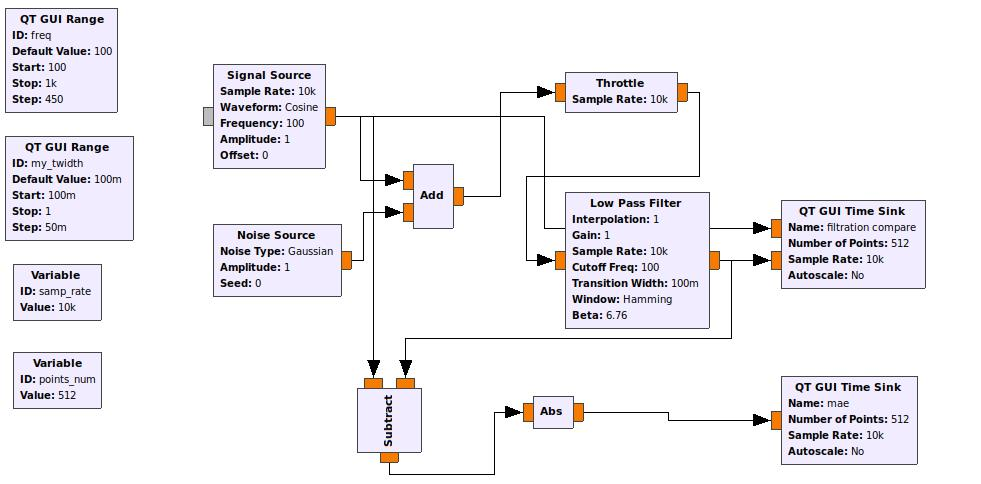
\includegraphics[scale=0.7]{block_schema}
		\caption{Блок-схема}
		\label{pic:block_schema} % название для ссылок внутри кода
	\end{center}
\end{figure}

\subsection{Исходный зашумленный сигнал}
\begin{figure}[H]
	\begin{center}
		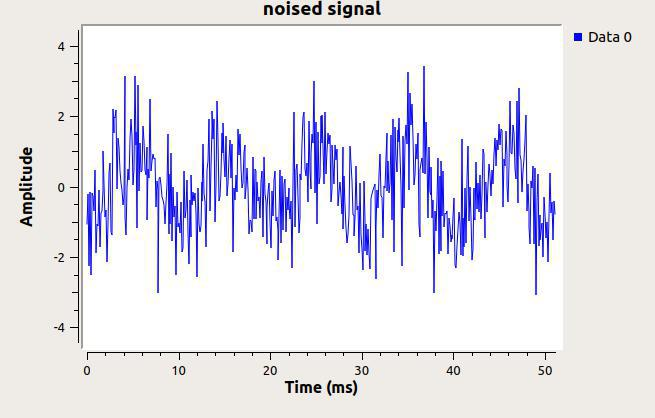
\includegraphics[scale=0.7]{noise_init}
		\caption{Исходный зашумленный сигнал}
		\label{pic:noise_init} % название для ссылок внутри кода
	\end{center}
\end{figure}
\newpage

% ------------------------------- init block -------------------------------------------
\subsection{Результаты фильтрации до настройки фильтра}
\begin{figure}[H]
	\begin{center}
		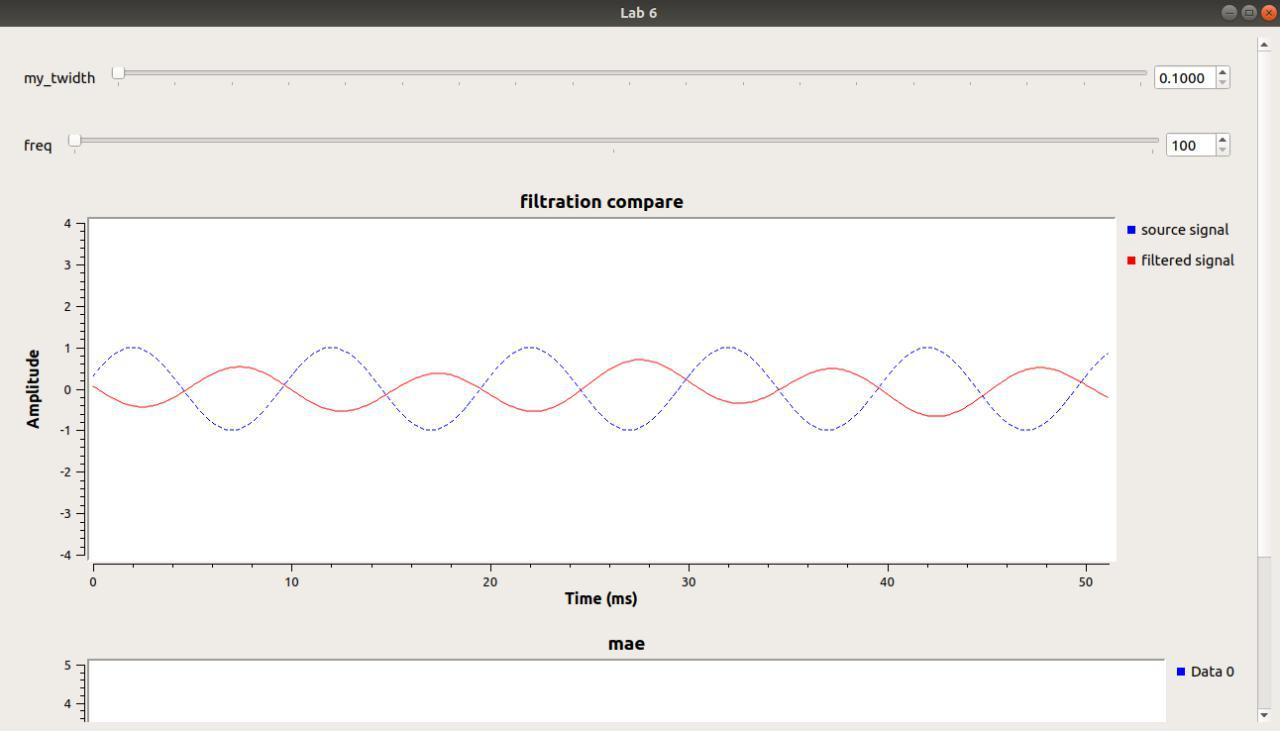
\includegraphics[scale=0.5]{graphic_init}
		\caption{Исходный и отфилтрованный зашумленный сигнал}
		\label{pic:graphic_init} % название для ссылок внутри кода
	\end{center}
\end{figure}

\begin{figure}[H]
	\begin{center}
		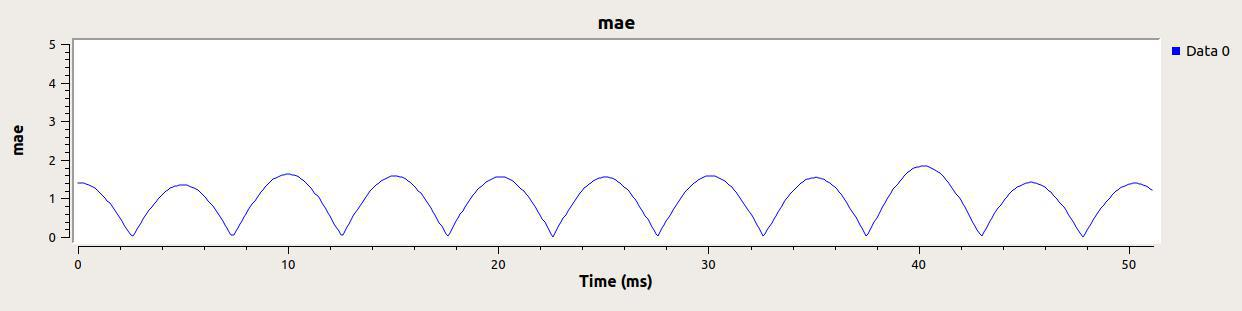
\includegraphics[scale=0.5]{mae_init}
		\caption{Средняя абсолютная ошибка}
		\label{pic:mae_init} % название для ссылок внутри кода
	\end{center}
\end{figure}
\newpage
% ------------------------------- edited block 1 -------------------------------------------
\subsection{Результаты филтрации с хорошо подоборанным параметром transition width}
\begin{figure}[H]
	\begin{center}
		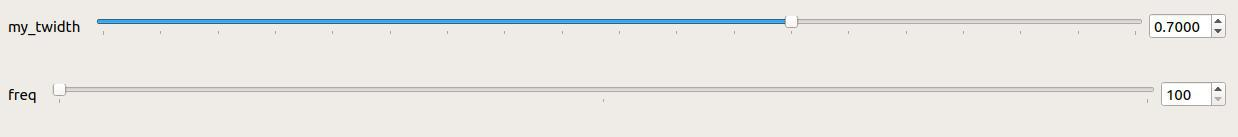
\includegraphics[scale=0.5]{good_params}
		\caption{Значение параметра transation width}
		\label{pic:good_params} % название для ссылок внутри кода
	\end{center}
\end{figure}


\begin{figure}[H]
	\begin{center}
		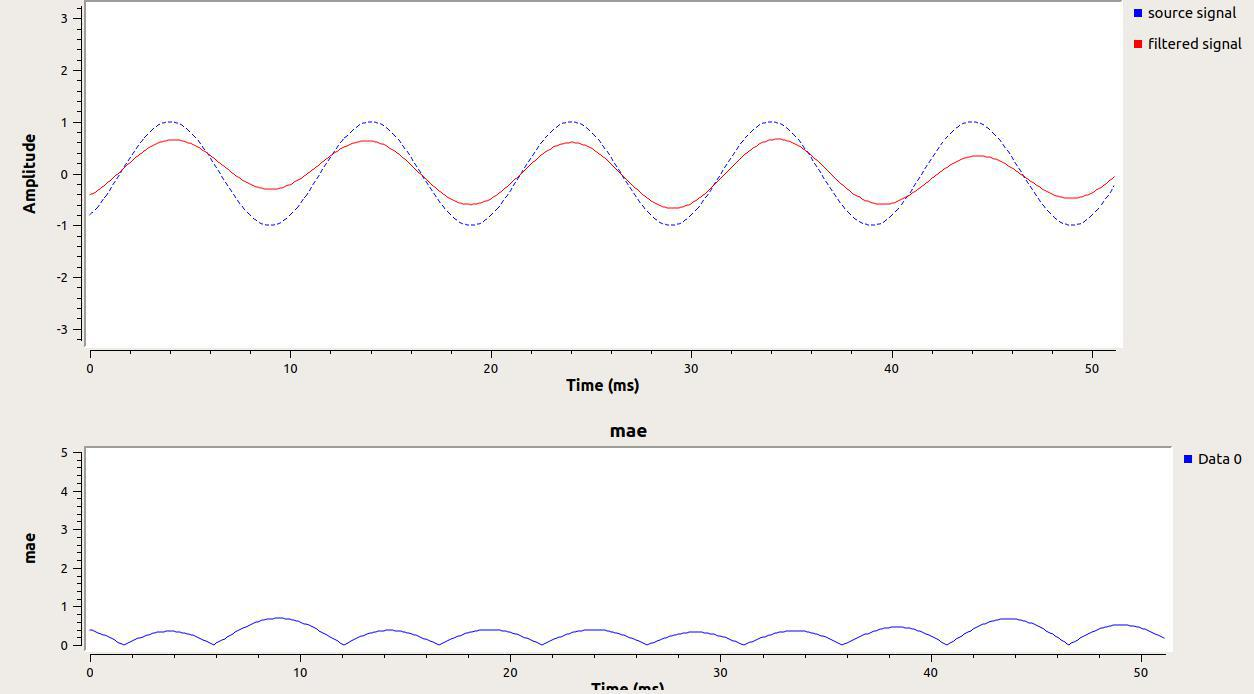
\includegraphics[scale=0.5]{good_graphics}
		\caption{Исходный сигнал, отфилтрованный зашумленный сигнал и средняя абсолютная ошибка}
		\label{pic:good_graphics} % название для ссылок внутри кода
	\end{center}
\end{figure}
\newpage

% ------------------------------- edited block 2 -------------------------------------------
\subsection{Результаты филтрации с плохо подоборанным параметром transition width}
\begin{figure}[H]
	\begin{center}
		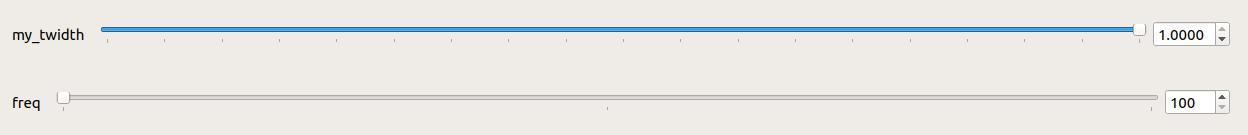
\includegraphics[scale=0.5]{bad_params}
		\caption{Значение параметра transation width}
		\label{pic:bad_params} % название для ссылок внутри кода
	\end{center}
\end{figure}


\begin{figure}[H]
	\begin{center}
		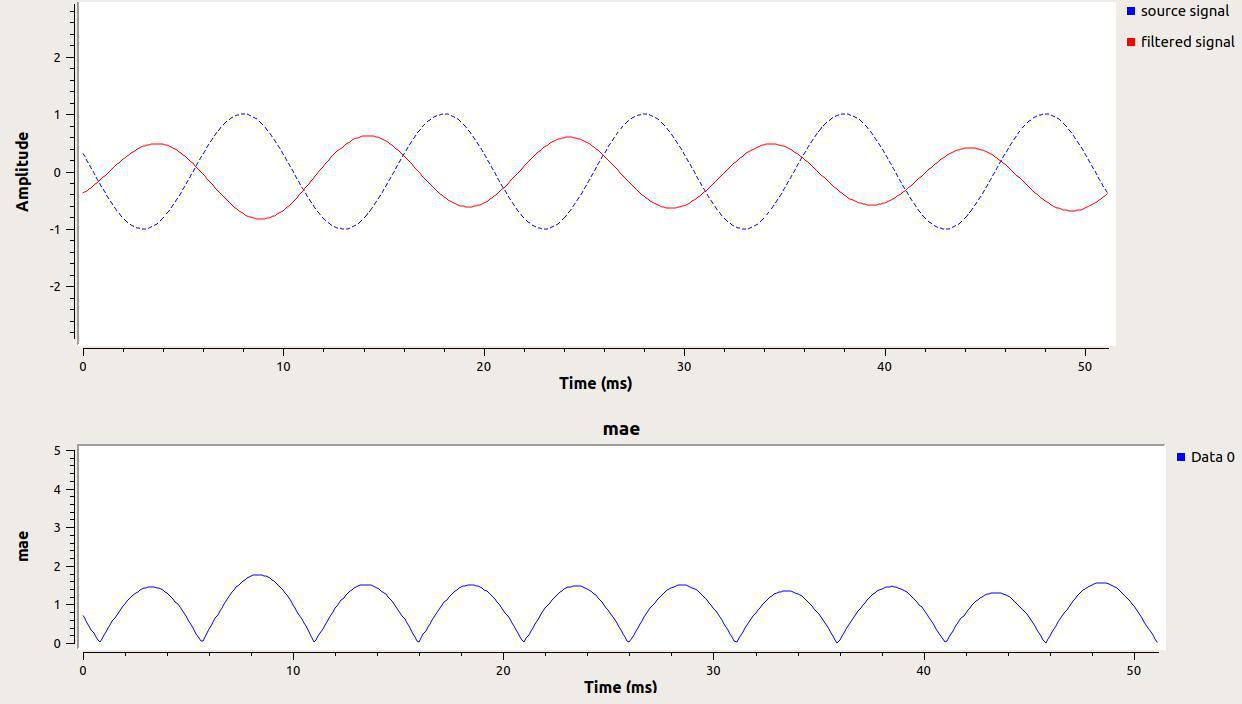
\includegraphics[scale=0.5]{bad_graphics}
		\caption{Исходный сигнал, отфилтрованный зашумленный сигнал и средняя абсолютная ошибка}
		\label{pic:bad_graphics} % название для ссылок внутри кода
	\end{center}
\end{figure}
\newpage

% ------------------------------- init block -------------------------------------------

\section{Выводы}

В данной работе были изучены основные возможности библиотеки gnuradio, была произведенна фильтрация зашумленного сигнала и интерактивная настройка фильтра в графической среде библиотеки gnuradio.
\end{document}
